\section{Production and information processes}

Porter's concept of information intensity and IT diversity helps explain how different industries rely on information and technology:
\begin{enumerate}
    \item Information intensity refers to the amount and complexity of information required in an organization's processes. 
     Generally, service industries require higher information intensity than manufacturing.
    \item IT Intensity measures how well IT systems meet an organization's information processing needs. 
        IT intensity is higher in banking than in insurance due to the industry's reliance on real-time transactions and data analysis.
        However, IT intensity can sometimes be greater in manufacturing than in services, depending on automation and digital integration.
    \item Management inclination reflects how much a company's leadership views IT as a strategic asset. 
        This varies based on factors like digital literacy, organizational culture, and company history.
        Historically, manufacturing companies have adopted IT earlier, while service industries experienced a lag of around ten years.
\end{enumerate}

\paragraph*{Information technology drivers}
Several factors determine how IT-intensive a company or industry can be:
\begin{enumerate}
    \item \textit{Structure of information processes}: the more structured and rule-based an activity is, the easier it is to automate using IT.
    \item \textit{Data volume}: the sheer amount of information that needs to be processed influences IT requirements.
    \item \textit{Operational frequency}: tasks that are repeated frequently benefit more from IT automation.
    \item \textit{Computational complexity}: simpler processes are easier to digitize and automate efficiently.
\end{enumerate}

\paragraph*{Porter's value chain}
Porter’s value chain concept highlights how IT supports various business activities to create competitive advantages.
\begin{figure}[H]
    \centering
    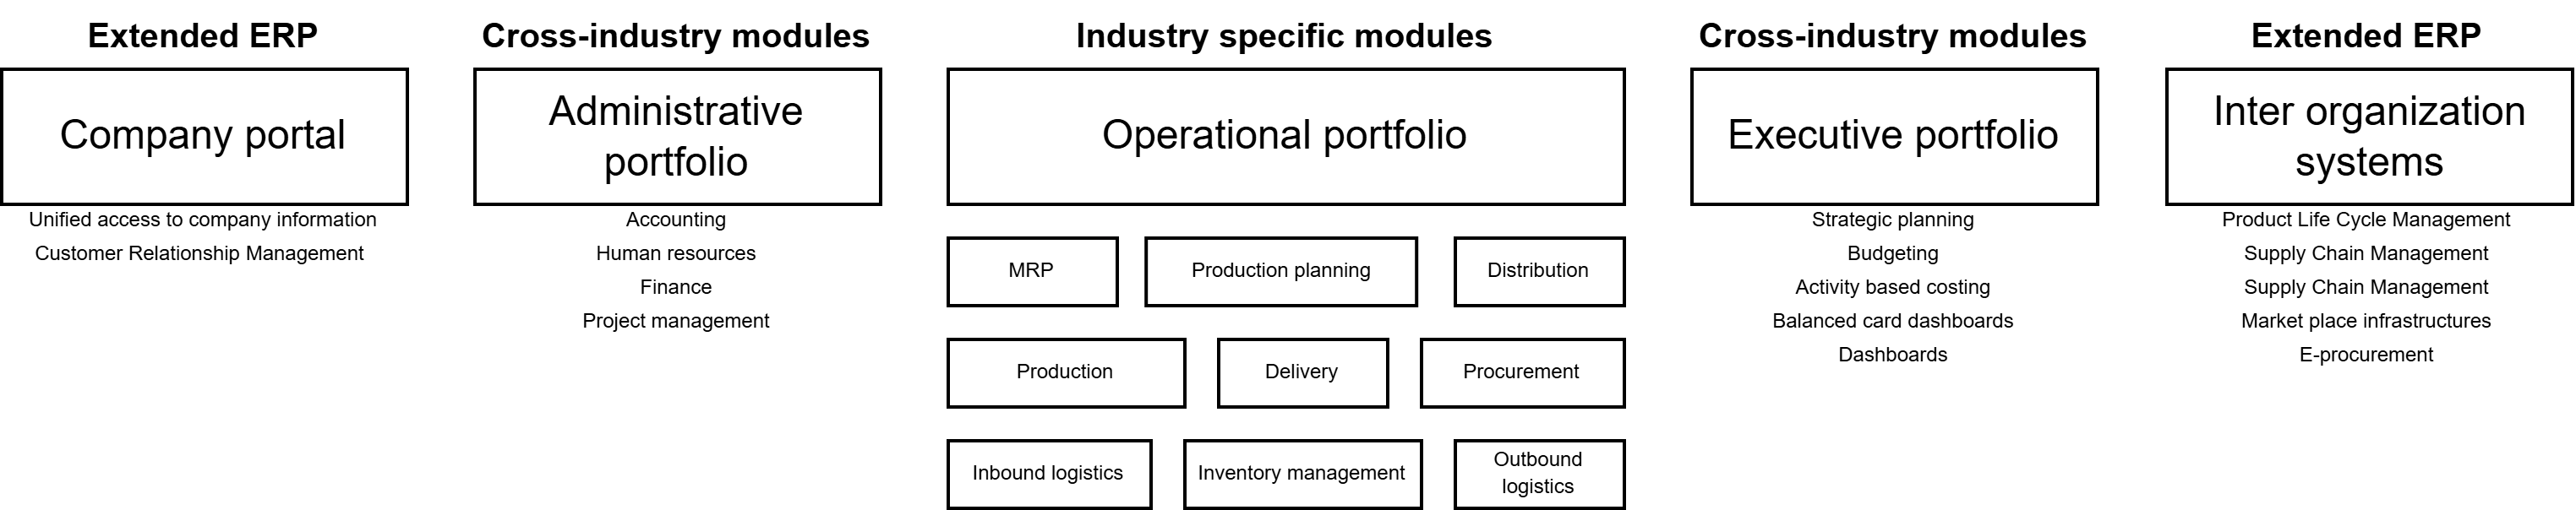
\includegraphics[width=0.5\linewidth]{images/bis1.png}
    \caption{Porter value chain}
\end{figure}

\paragraph*{Activity cycles}
Manufacturing involves continuous, iterative cycles that ensure efficiency and product quality. 
These cycles include:
\begin{enumerate}
    \item \textit{Development cycle}: focuses on designing and industrializing both products and production processes.
    \item \textit{Logistics cycle}: manages customer orders through:
        \begin{itemize}
            \item \textit{Procurement}: acquiring and handling materials, including reception, warehousing, and distribution to production plants.
            \item \textit{Production}: the physical transformation of raw materials into finished goods.
            \item \textit{Sales and distribution}: managing orders, external logistics, and post-sale services such as maintenance and customer support.
        \end{itemize}
\end{enumerate}